\chapter{Introduction}
\label{chap:introduction}
In the traditional sense, harmonic analysis relates to a set of music theory studies that pretend to describe the relationship of simultaneous sonorities and generalize rules of how each of these sonorities should move to facilitate and embellish their combined sound.

\section{Motivation}
Students at conservatoires often learn the guidelines of harmonic analysis during a specialized course of Harmony. Such a course could extend to several years, making it a difficult subject to be learnt fast for a beginner. Even in the case of experts, it might take relatively long time to analyze a piece of music in terms of harmony, which makes the task of automating it valuable even for the expert theorist.

% I could add examples of harmonic reduction, transcription, and other uses
% However, this has low priority.

It is difficult, however, to give a precise definition of what is harmonic analysis and where the task of automatic harmonic analysis begins and ends. As will be discussed in \autoref{chap:literature-review}, different researchers have made different characterizations of the problem, sometimes binding these characterizations closely to the mathematical tools they have used to approach the problem, in other cases to the type of music that they pretend to analyze, and in other cases due to other circumstances. For this particular work, I intend to define harmonic analysis based in two simple definitions, and afterwards, the outcome definition will help to describe which are the expected inputs and outputs of an automatic harmonic analysis system.

\section{Harmonic analysis}
According to the Oxford Music Online dictionary, in the context of music, the term \emph{analysis} could be defined as the following: \cite{oxfordanalysis}

\begin{quote}
\centering
\emph{[...] the interpretation of structures in music, \linebreak
their resolution into relatively simpler constituent elements, \linebreak and the investigation of the relevant functions of those elements.}
\end{quote}

Additionally, according to the same source, a very simplistic definition of harmony could be: \cite{oxfordharmony}

\begin{quote}
\centering
\emph{The simultaneous sounding (i.e. combination) of notes [...]}
\end{quote}

\begin{figure}[h]
  \centering
    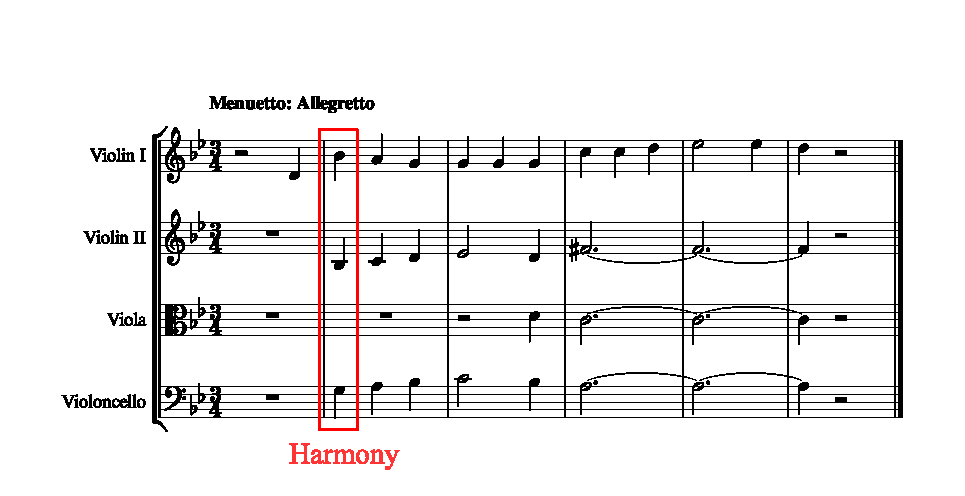
\includegraphics[width=1.0\textwidth]{01-introduction/figures/1}
  \caption{Excerpt from Joseph Haydn's Op.20 No.3 - II. Menuetto: Allegretto, mm. 1-6}
  \label{fig:harmony}
\end{figure}

Combining these definitions, one possible interpretation of what is a harmonic analysis could be the following:

\begin{quote}
\centering
\emph{[...] the interpretation of \textbf{harmonic} structures in music,
their resolution into relatively simpler constituent elements, \textbf{i.e., harmonic labels}, and the investigation of the relevant functions of those \textbf{labels}.}
\end{quote}

\begin{figure}[h]
  \centering
    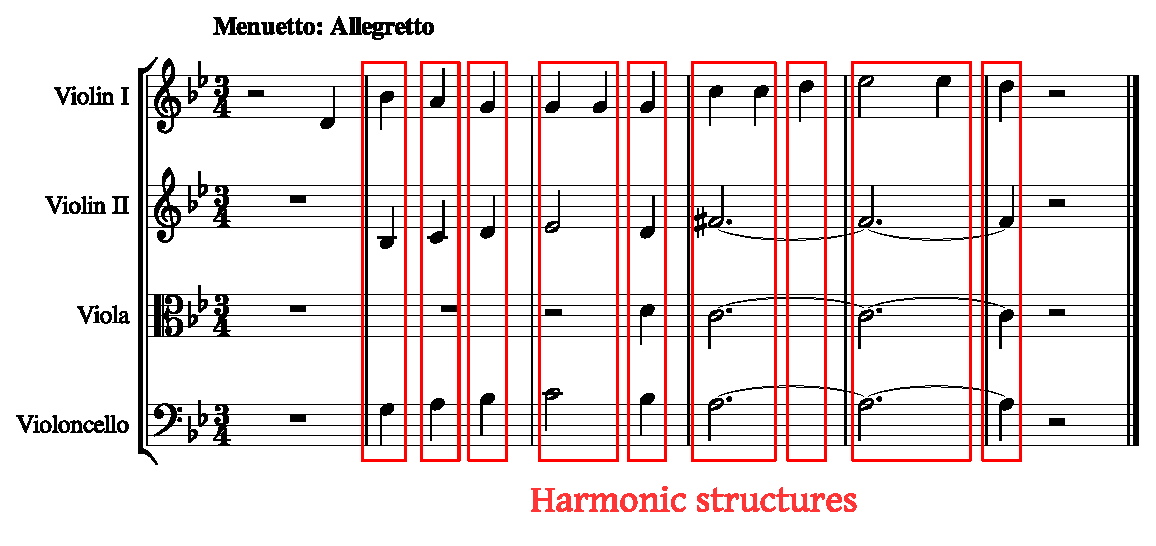
\includegraphics[width=1.0\textwidth]{01-introduction/figures/2}
  \caption{Highlighting harmonic structures in musical excerpt}
  \label{fig:harmonic-structures}
\end{figure}

Therefore, as stated by this definition, the process of harmonic analysis comprises three steps:

\begin{itemize}
  \item Interpret harmonic structures
  \item Resolve them into harmonic labels
  \item Investigate their relevant functions
\end{itemize}

For breaking down the steps of the analysis, we could use a fragment of a musical score. \autoref{fig:harmony} remarks the first beat of the second measure, where three instruments play notes together. Every instance of these simultaneities represents harmony. If these harmonies are clustered and interpreted, we come up with harmonic structures, as in  \autoref{fig:harmonic-structures}.

In order to satisfy the second step of harmonic analysis, we could resolve this interpretation of harmonic structures into some sort of simpler representation. Historically, music theorists performing these sort of harmonic analysis will most likely come with a system of labels that represent the meaning of the harmonic structures. There is not a single labeling system for this purpose. \autoref{fig:harmonic-labels} shows three possible representations for the harmonic structures of the same music excerpt presented previously.

\begin{figure}[h]
  \centering
    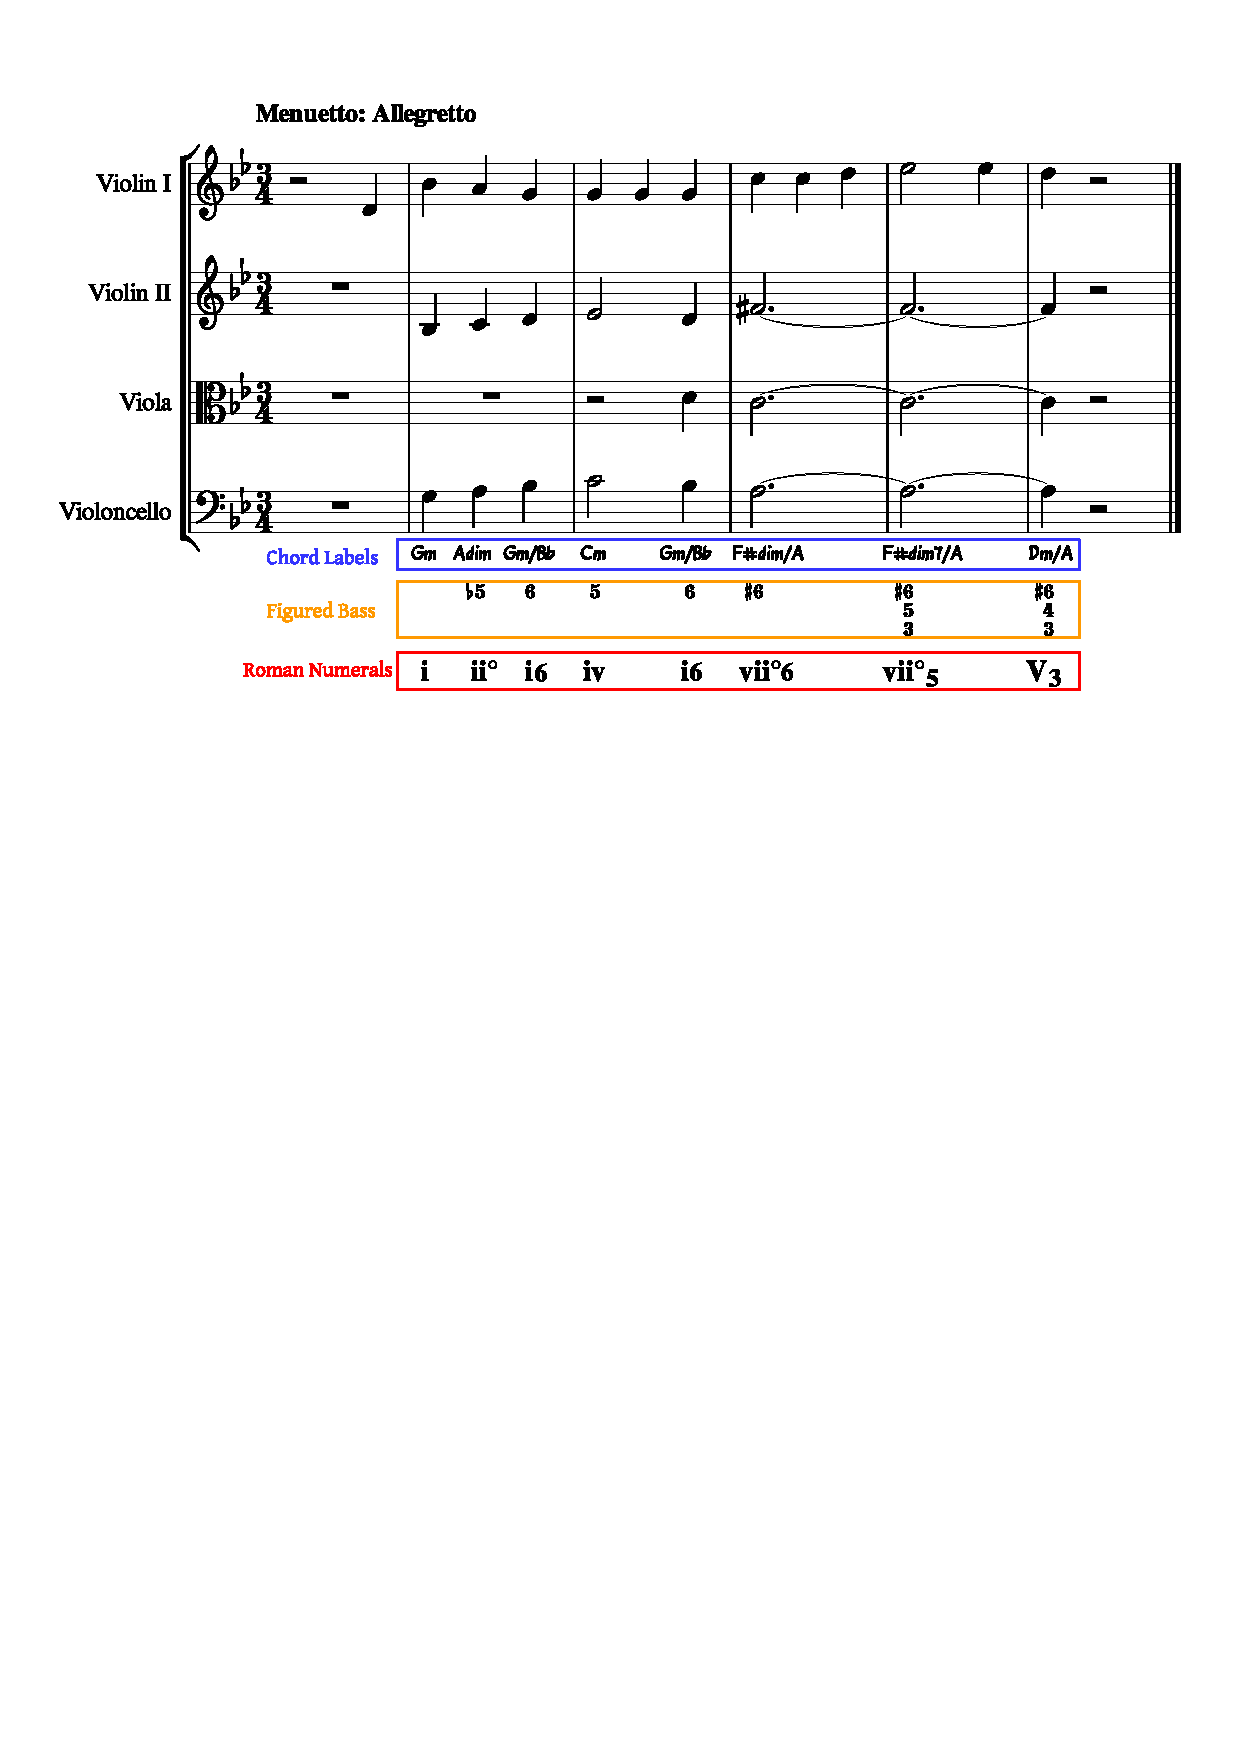
\includegraphics[width=1.0\textwidth]{01-introduction/figures/3}
  \caption{Three different harmonic labeling representations of a musical fragment}
  \label{fig:harmonic-labels}
\end{figure}

Any of these three representations would suffice the second step of harmonic analysis. The chord labels in the first representation are what is commonly seen to label harmonic structures in jazz and pop music. The figured bass from the second representation was very popular previous to the classical period, and it was intended to aid accompanyists who played in chamber ensembles, e.g., it helped a harpsichordist to "fill-in" the accompaniment during the performance when only one note was given in the score. The third representation using roman numerals emerged previously but consolidated with the theoretical work of Hugo Riemann, and its purpose is mainly of analysis. For this work, I have selected to use the third kind of representation, because it is the one that helps the better in the third step of the process, \emph{specifying the function of the harmonic labels}.

In fact, it could be claimed that in the roman numeral labels themselves, the whole process of harmonic analysis gets summarized, as the clustering and interpretation of harmonic structures will be characterized by the appearance of harmonic labels, and in the case of roman numeral labels, the function of that harmonic structure is implicitly given by the roman numeral degree.

\section{Automatic harmonic analysis}
Once the steps in the process of performing a harmonic analysis and the selected labels for harmonic structures are specified, I will now define a system of automatic harmonic analysis as a piece of software that given a fragment of music as input, will output the same piece of music, with roman numeral labels appended to it, as \autoref{fig:automatic-harmonic-analysis} shows.

\begin{figure}[h]
  \centering
    \includegraphics[width=1.0\textwidth]{01-introduction/figures/4}
  \caption{A system of automatic harmonic analysis}
  \label{fig:automatic-harmonic-analysis}
\end{figure}

There is, however, the problem of choosing among the multiple ways in which this score can be represented. For this work, a symbolic representation in the \emph{humdrum} \cite{humdrum} format was chosen as the input format for this system. Similarly, the output consists of the same humdrum representation with an additional spine in the \emph{**harm} \cite{harm} syntax. The justification behind this decision will be described in \autoref{chap:dataset}.

% \section{Objectives}
% This work pretends to reproduce and apply the current approach for automatic functional harmonic analysis used over the KernScores corpora, and apply it to a specific set of string quartets from Joseph Haydn. Once these automatic analyses are performed, they will be compared to manual annotations over the same set of string quartets.
%
% \section{Structure of the Report}
% Literature. Methods. Results. Discussion.

\newpage
